We present here a table summarizing the performance results obtained for the OCL
operations on collections.

\newpage
\begin{longtable}{ c|c c c c}
  \textbf{Operation} & \textbf{Sequence} & \textbf{Set} & \textbf{Bag} & \textbf{OrderedSet} \\\hline
  allInstances & 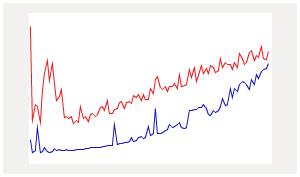
\includegraphics[width=1.6cm]{../graphs/AllInstances} & & &
  \\\hline  

any
&
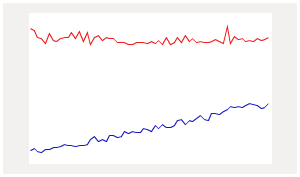
\includegraphics[width=1.6cm]{../graphs/sequence/small/Any} 
&
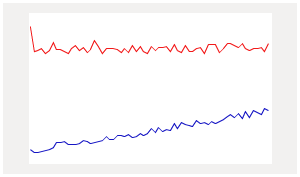
\includegraphics[width=1.6cm]{../graphs/set/small/Any}
& 
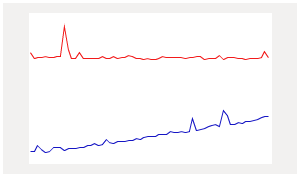
\includegraphics[width=1.6cm]{../graphs/bag/small/Any}
& 
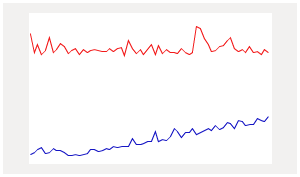
\includegraphics[width=1.6cm]{../graphs/orderedset/small/Any}
\\\hline
  
append
& 
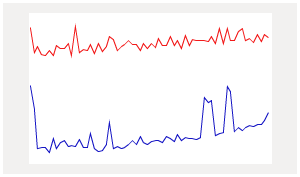
\includegraphics[width=1.6cm]{../graphs/sequence/small/Append}
&
&
& 
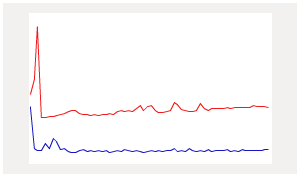
\includegraphics[width=1.6cm]{../graphs/orderedset/small/Append}
\\\hline
  
at
& 
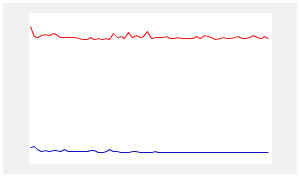
\includegraphics[width=1.6cm]{../graphs/sequence/small/At}
&
&
& 
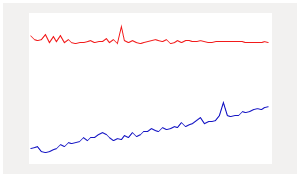
\includegraphics[width=1.6cm]{../graphs/orderedset/small/At}
\\\hline

collect
&
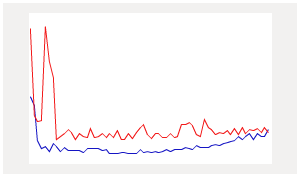
\includegraphics[width=1.6cm]{../graphs/sequence/small/Collect} 
&
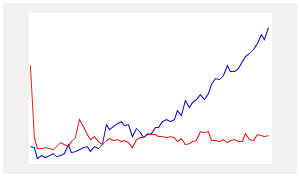
\includegraphics[width=1.6cm]{../graphs/set/small/Collect}
&
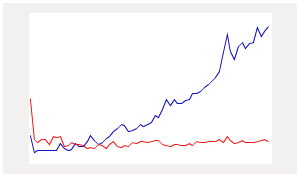
\includegraphics[width=1.6cm]{../graphs/bag/small/Collect}
&
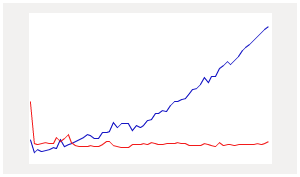
\includegraphics[width=1.6cm]{../graphs/orderedset/small/Collect}
\\\hline

eq
&
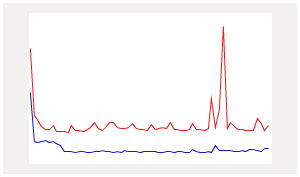
\includegraphics[width=1.6cm]{../graphs/sequence/small/EQ}
&
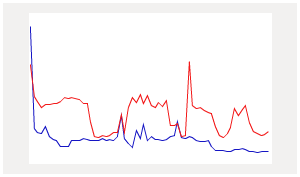
\includegraphics[width=1.6cm]{../graphs/set/small/EQ}
&
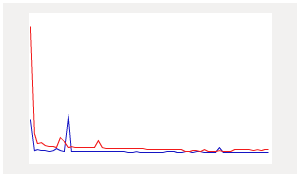
\includegraphics[width=1.6cm]{../graphs/bag/small/EQ}
&
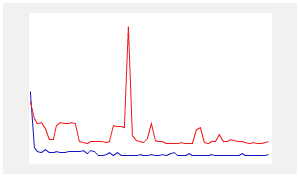
\includegraphics[width=1.6cm]{../graphs/orderedset/small/EQ}
\\\hline

excludes
&
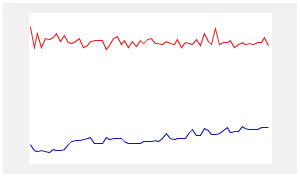
\includegraphics[width=1.6cm]{../graphs/sequence/small/Excludes}
&
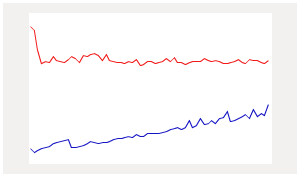
\includegraphics[width=1.6cm]{../graphs/set/small/Excludes}
&
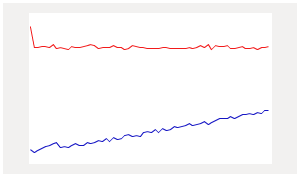
\includegraphics[width=1.6cm]{../graphs/bag/small/Excludes}
&
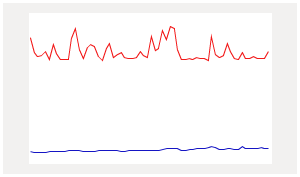
\includegraphics[width=1.6cm]{../graphs/orderedset/small/Excludes}
\\\hline

excludesAll
&
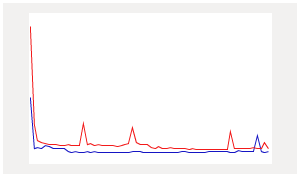
\includegraphics[width=1.6cm]{../graphs/sequence/small/ExcludesAll}
&
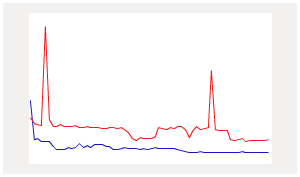
\includegraphics[width=1.6cm]{../graphs/set/small/ExcludesAll}
&
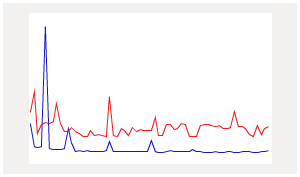
\includegraphics[width=1.6cm]{../graphs/bag/small/ExcludesAll}
&
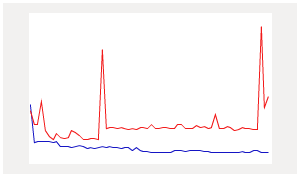
\includegraphics[width=1.6cm]{../graphs/orderedset/small/ExcludesAll}
\\\hline

excluding
&
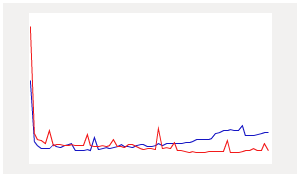
\includegraphics[width=1.6cm]{../graphs/sequence/small/Excluding}
&
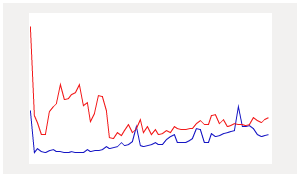
\includegraphics[width=1.6cm]{../graphs/set/small/Excluding}
&
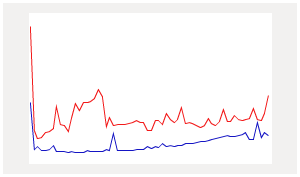
\includegraphics[width=1.6cm]{../graphs/bag/small/Excluding}
&
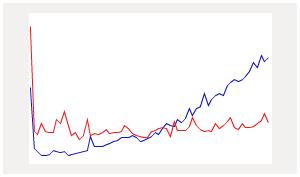
\includegraphics[width=1.6cm]{../graphs/orderedset/small/Excluding}
\\\hline

exists
&
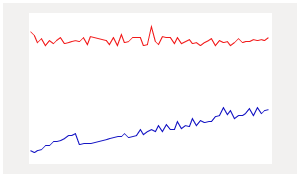
\includegraphics[width=1.6cm]{../graphs/sequence/small/Exists}
&
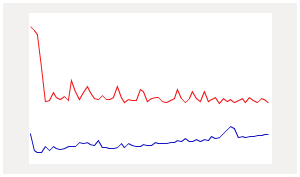
\includegraphics[width=1.6cm]{../graphs/set/small/Exists}
&
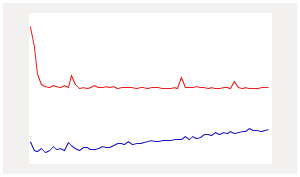
\includegraphics[width=1.6cm]{../graphs/bag/small/Exists}
&
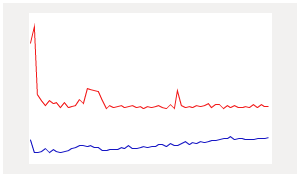
\includegraphics[width=1.6cm]{../graphs/orderedset/small/Exists}
\\\hline

first
&
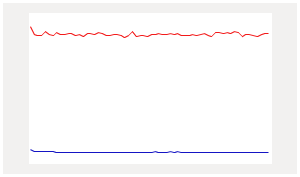
\includegraphics[width=1.6cm]{../graphs/sequence/small/First}
&
&
&
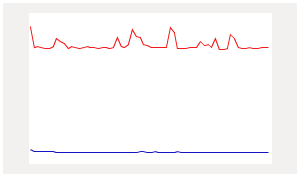
\includegraphics[width=1.6cm]{../graphs/orderedset/small/First}
\\\hline

flatten
&
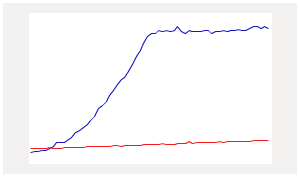
\includegraphics[width=1.6cm]{../graphs/sequence/small/Flatten}
&
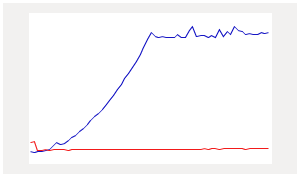
\includegraphics[width=1.6cm]{../graphs/set/small/Flatten}
&
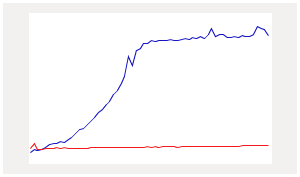
\includegraphics[width=1.6cm]{../graphs/bag/small/Flatten}
&
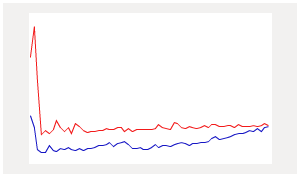
\includegraphics[width=1.6cm]{../graphs/orderedset/small/Flatten}
\\\hline

forAll
&
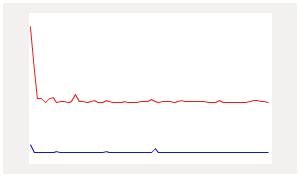
\includegraphics[width=1.6cm]{../graphs/sequence/small/forALL}
&
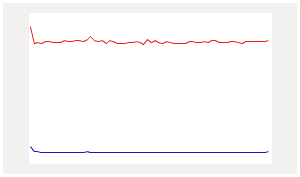
\includegraphics[width=1.6cm]{../graphs/set/small/forALL}
&
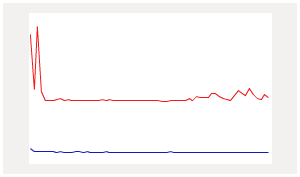
\includegraphics[width=1.6cm]{../graphs/bag/small/forALL}
&
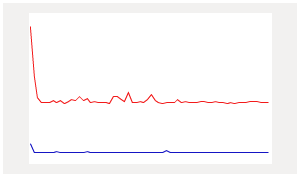
\includegraphics[width=1.6cm]{../graphs/orderedset/small/forALL}
\\\hline

includes
&
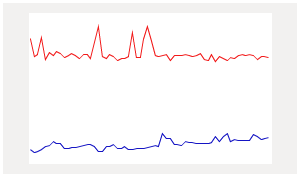
\includegraphics[width=1.6cm]{../graphs/sequence/small/Includes}
&
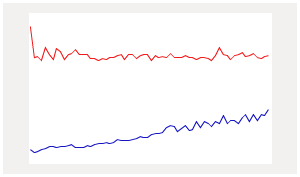
\includegraphics[width=1.6cm]{../graphs/set/small/Includes}
&
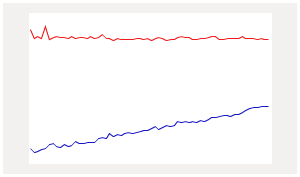
\includegraphics[width=1.6cm]{../graphs/bag/small/Includes}
&
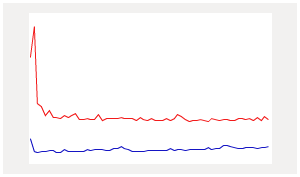
\includegraphics[width=1.6cm]{../graphs/orderedset/small/Includes}
\\\hline

includesAll
&
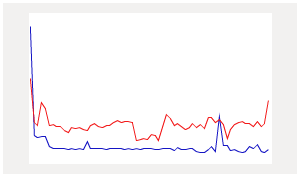
\includegraphics[width=1.6cm]{../graphs/sequence/small/IncludesAll}
&
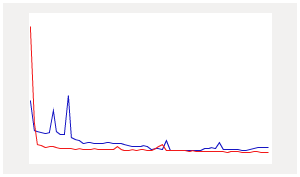
\includegraphics[width=1.6cm]{../graphs/set/small/IncludesAll}
&
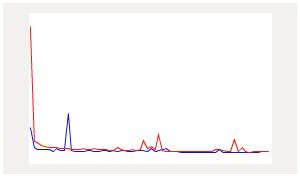
\includegraphics[width=1.6cm]{../graphs/bag/small/IncludesAll}
&
\includegraphics[width=1.6cm]{../graphs/orderedset/small/IncludesAll}
\\\hline

including
&
\includegraphics[width=1.6cm]{../graphs/sequence/small/Including}
&
\includegraphics[width=1.6cm]{../graphs/set/small/Including}
&
\includegraphics[width=1.6cm]{../graphs/bag/small/Including}
&
\includegraphics[width=1.6cm]{../graphs/orderedset/small/Including}
\\\hline

indexOf
&
\includegraphics[width=1.6cm]{../graphs/sequence/small/IndexOf}
&
&
&
\includegraphics[width=1.6cm]{../graphs/orderedset/small/IndexOf}
\\\hline

intersection
&
&
\includegraphics[width=1.6cm]{../graphs/set/small/Intersection}
&
&
\\\hline

insertAt
&
\includegraphics[width=1.6cm]{../graphs/sequence/small/InsertAt}
&
&
&
\includegraphics[width=1.6cm]{../graphs/orderedset/small/InsertAt}
\\\hline

isEmpty
&
\includegraphics[width=1.6cm]{../graphs/sequence/small/IsEmpty}
&
\includegraphics[width=1.6cm]{../graphs/set/small/IsEmpty}
&
\includegraphics[width=1.6cm]{../graphs/bag/small/IsEmpty}
&
\includegraphics[width=1.6cm]{../graphs/orderedset/small/IsEmpty}
\\\hline

isUnique
&
\includegraphics[width=1.6cm]{../graphs/sequence/small/isUnique}
&
\includegraphics[width=1.6cm]{../graphs/set/small/isUnique}
&
\includegraphics[width=1.6cm]{../graphs/bag/small/isUnique}
&
\includegraphics[width=1.6cm]{../graphs/orderedset/small/isUnique}
\\\hline

iterate
&
\includegraphics[width=1.6cm]{../graphs/sequence/small/Iterate}
&
\includegraphics[width=1.6cm]{../graphs/set/small/Iterate}
&
\includegraphics[width=1.6cm]{../graphs/bag/small/Iterate}
&
\includegraphics[width=1.6cm]{../graphs/orderedset/small/Iterate}
\\\hline

last
&
\includegraphics[width=1.6cm]{../graphs/sequence/small/Last}
&
&
&
\includegraphics[width=1.6cm]{../graphs/orderedset/small/Last}
\\\hline

minus
&
&
\includegraphics[width=1.6cm]{../graphs/set/small/Minus}
&
&
\\\hline

notEqual
&
\includegraphics[width=1.6cm]{../graphs/sequence/small/NEQ}
&
\includegraphics[width=1.6cm]{../graphs/set/small/NEQ}
&
\includegraphics[width=1.6cm]{../graphs/bag/small/NEQ}
&
\includegraphics[width=1.6cm]{../graphs/orderedset/small/NEQ}
\\\hline

one
&
\includegraphics[width=1.6cm]{../graphs/sequence/small/One}
&
\includegraphics[width=1.6cm]{../graphs/set/small/One}
&
\includegraphics[width=1.6cm]{../graphs/bag/small/One}
&
\includegraphics[width=1.6cm]{../graphs/orderedset/small/One}
\\\hline

prepend
&
\includegraphics[width=1.6cm]{../graphs/sequence/small/Prepend}
&
&
&
\includegraphics[width=1.6cm]{../graphs/orderedset/small/Prepend}
\\\hline

reject
&
\includegraphics[width=1.6cm]{../graphs/sequence/small/Reject}
&
\includegraphics[width=1.6cm]{../graphs/set/small/Reject}
&
\includegraphics[width=1.6cm]{../graphs/bag/small/Reject}
&
\includegraphics[width=1.6cm]{../graphs/orderedset/small/Reject}
\\\hline

select
&
\includegraphics[width=1.6cm]{../graphs/sequence/small/Select}
&
\includegraphics[width=1.6cm]{../graphs/set/small/Select}
&
\includegraphics[width=1.6cm]{../graphs/bag/small/Select}
&
\includegraphics[width=1.6cm]{../graphs/orderedset/small/Select}
\\\hline

size
&
\includegraphics[width=1.6cm]{../graphs/sequence/small/Size}
&
\includegraphics[width=1.6cm]{../graphs/set/small/Size}
&
\includegraphics[width=1.6cm]{../graphs/bag/small/Size}
&
\includegraphics[width=1.6cm]{../graphs/orderedset/small/Size}
\\\hline

sortedBy
&
\includegraphics[width=1.6cm]{../graphs/sequence/small/sortedBy}
&
\includegraphics[width=1.6cm]{../graphs/set/small/sortedBy}
&
\includegraphics[width=1.6cm]{../graphs/bag/small/sortedBy}
&
\includegraphics[width=1.6cm]{../graphs/orderedset/small/sortedBy}
\\\hline

subOrderedSet 
&
&
&
&
\includegraphics[width=1.6cm]{../graphs/orderedset/small/Suborderedset}
\\\hline

subSequence
&
\includegraphics[width=1.6cm]{../graphs/sequence/small/SubSequence}
&
&
&
\\\hline

sum
&
\includegraphics[width=1.6cm]{../graphs/sequence/small/Sum}
&
\includegraphics[width=1.6cm]{../graphs/set/small/Sum}
&
\includegraphics[width=1.6cm]{../graphs/bag/small/Sum}
&
\includegraphics[width=1.6cm]{../graphs/orderedset/small/Sum}
\\\hline

symmetricDifference
&
&
\includegraphics[width=1.6cm]{../graphs/set/small/SymmetricDif}
&
&
\\\hline

union
&
\includegraphics[width=1.6cm]{../graphs/sequence/small/Union}
&
\includegraphics[width=1.6cm]{../graphs/set/small/Union}
&
&
\includegraphics[width=1.6cm]{../graphs/orderedset/small/Union}
\\\hline

\caption{Evaluation Results }
\label{tab:resultsFull}
\end{longtable}


